\chapter{The Standard Model and Left-Right Symmetric Extensions}
\label{chapter:lrsm}

I wonder if I want to write something here?

\section{Evolution of the Standard Model}
\label{sec:lrsm:history}

This section is about the history of the Standard Model. Huh.
\cref{fig:sm} displays the known elementary particles.

\begin{figure}
    \centering
    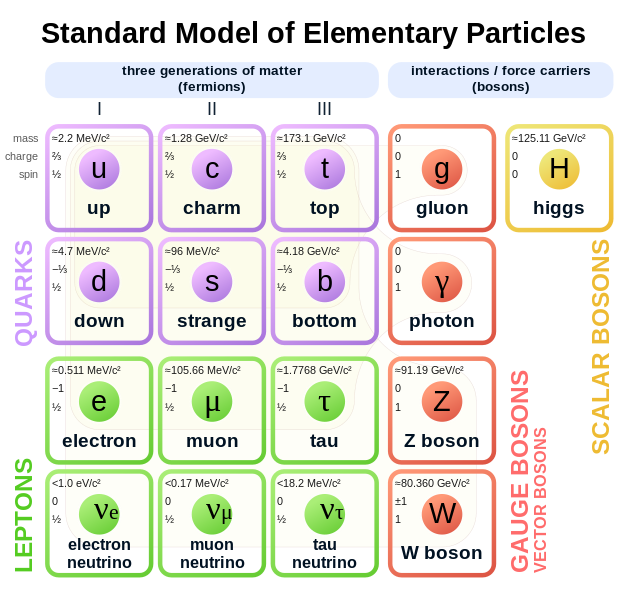
\includegraphics[width=\textwidth]{figures/intro/Standard_Model_of_Elementary_Particles.svg.png}
    \caption{
      The Standard Model of Particle Physics showing the twelve fermions and five bosons,
      their various properities (mass, charge, spin), labels (box and circle colors),
      and interactions (brown loops). Credit to Cush on wikipedia for
      providing this diagram freely accessible and usable for any purpose.
    }
    \label{fig:sm}
  \end{figure}

\section{The Standard Model Landscape}

Hi my name is Billy.

\subsection{Quantum Chromodynamics and the Strong Force}

Hi my name is Billy.
